\subsection{Relativistic Heavy Ion Collision Phenomenology}
Heavy ion collisions can be described in terms of a sequences of states that the system is in over time, beginning with the initial state of the colliding nuclei and ending with the final state partcles produced in the collision.
The system goes through extreme changes in energy density and temperature through this evolution, therefore the system is best modeled through a combination of phenomenological models. 
Figure~\ref{fig:heavy_ion_collision_evolution} shows a schematic of the phenomenological models used to describe the heavy ion collision evolution.

\begin{figure}
    \centering
    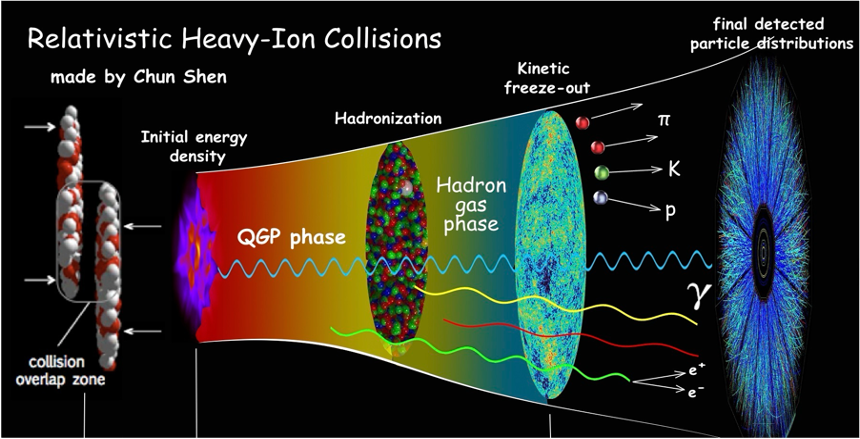
\includegraphics[width=\textwidth]{figures/chapter1/hic_phenomenology.png}
    \caption{Schematic of the phenomenological models used to describe the heavy ion collision evolution: initial state, thermalization, hydrodynamic evolution, hadronization, and freeze-out. Reproduced from \cite{heavy_ion_collision_evolution}.}
    \label{fig:heavy_ion_collision_evolution}
\end{figure}

The initial state of heavy ion collisions can be described in a variety of ways using phenomenological models, including the models outlined in Section~\ref{sec:qgp}.
Additional models include kinetic gas theories, string models, and glasma models for the initial state.
Following the initial state modeling at a set time from the collision, the system undergoes a thermalization process where the system is assumed to reach local thermal equilibrium.
At this point, the system can be described by a hydrodynamical model where the system is treated as a relativistic fluid.
Here, the QGP phase is modeled using a variety of equations of state and viscoity terms as the system expands and cools.
In practice, the system is evolved hydrodynamically by evolving the energy density and velocity field of hypercube lattices.

Once the hypercubes on the surface of the fluid system reach a low enough energy density or temperature, they are each hadronized locally using the Cooper-Frye method which samples a distribution of particles from these fluid cells assuming a grand canonical ensemble of particle states.
The resulting hadrons are then developed through a particle cascade where elastic and inelastic collisions and particle decays are simulated.
Finally, the system is frozen out and the final state particles are available for analysis and comparison to experimental data.
A suite of light weight ion collision event generators are used to model this evolution of the heavy ion collision system including some or all of these steps.
Descritions of the set of event generators used for comparison to and extraction of truth level information from experimental data for the analyses in this thesis are included in the following sections.

\subsection{Monte Carlo Generators in Au+Au analysis}
\subsubsection{\hijing}
\hijing (Heavy Ion Jet Interaction Generator) is a Monte Carlo event generator designed for simulating high-energy heavy-ion and proton-proton collisions and is used in this thesis for simulating a set of minimum bias Au+Au collisions at 200 GeV. 
\hijing uses the Glauber model to describe the geometry of the colliding nuclei and perturbative QCD to model hard scatterings as minijets, where a scale pTmin can be used to determine whether an interaction is considered "hard" or "soft."
Multi-parton interactions, initial state radiation, and final state radiation are also included in the modeling through this minijet production.
Soft interactions are modeled using the Dual Parton Model (DPM), where the colliding nucleons are represented as color strings.
Both the hard and soft interactions modeled within \hijing are then hadronized into final-state particles using the Lund string model.
Noteably, while \hijing models both the initial stage hard and soft iteractions and the hadronization stage of heavy ion collisions, \hijing does not include a hydrodynamic evolution stage or allow for coalescence within its hadronization stage, and thus does not fully model the known processes of the QGP phase of heavy ion collision.
To account for this, collective flow effects are added to the final state particle distribution in \hijing via an afterburner within the sPHENIX simulation framework.

\subsubsection{\ampt}
\ampt (A Multi-Phase Transport Model) is a Monte Carlo event generator that simulates heavy-ion collisions by modeling multiple stages of the collision process, including the initial parton production, parton transport, hadronization, and hadronic interactions.
\ampt has a similar theoretical basis to \hijing and uses \hijing to generate the initial parton distribution; these partons are then developed through a parton cascade of 2-2 elastic collisions, where the strength of parton interactions determines the transport properties of the QGP.
\textcolor{red}{Do these transport properties mean viscosity, so flow effects should be included?}
Hadronization is then modeled using a quark coalescence model. 
Finally, the resulting hadron distribution is developed through a hadron transport model that includes elastic and inelastic scatterings, and resonance decays, to model interactions before the system's kinetic freeze out.
\subsubsection{\epos}
\epos (Energy conserving quantum mechanical multiple scattering approach, based on Partons (parton ladders), Off-shell remnants, Splitting of parton ladders) uses an entirely different approach to modeling the inital stage of heavy ion collisions then \hijing and \ampt.
\epos models collisions using an S-matrix approach to Gribov-Regge Theory which simultaneously describes soft and hard scatterings. 
\textcolor{red}{Include diagram of parton ladder and also another sentence explaining this.}
Primary interactions are developed based on this S-matrix approach for parallel scatterings, then the system undergoes a core-corona separation procedure where the core (high-density region) first undergoes hydrodynamic evolution then hadronization and the corona (low-density region) is treated as independent strings and hadronized using the Lund string model.
In the core, initial conditions of the hydrodynamic modeling (energy density, velocity, conserved charges) are determined from the dense parton strings and the system is evolved using 3D+1 hydrodynamics with a realistic equation of state and viscoity terms.
Finally, these hydrodynamic fluid cells are hadronized using the Cooper-Frye method which assume a grand canonical ensemble and the resulting hadrons are the developed through a hadronic cascade where similar to \ampt, elastic and inelastic collisions and particle decays are simulated. 
\subsection{Monte Carlo Generators in p+p analysis}
\subsubsection{\pythia}
\pythia is a very widely used Monte Carlo event generator for simulating high-energy particle collisions, particularly in proton-proton interactions.
The initial hard scattering is modeled using parton distribution functions to describe the distribution of quarks and glouns within the colliding protons and perturbative QCD to model the hard scattering process.
Parton showers are then simulated to account for initial state radiation (ISR) and final state radiation (FSR). 
Multiple parton interactions (MPI) are also included to model the possibility of multiple hard scatterings occurring in a single proton-proton collision.
\textcolor{red}{Include sentence on how MPI are modeled in \pythia, eikonal MPI}.
\textcolor{red}{Include figure of pythia evolution scheme, showing how ISR/FSR/MPI are interleaved.}
In \pythia, the underlying event contributions (ISR/FSR/MPI) are evolved together using a pT-ordered showing scheme, where the hardest interaction is evolved first and softer interactions are evolved later, and the evolution is interleaved to allow for competition between ISR, FSR, and MPI.
Hadronization is modeled using the Lund string fragmentation model, where color strings are formed between partons and then break into hadrons.
\pythia also includes a variety of tunable parameters that can be adjusted to better match experimental data, a \pythia tune developed for RHIC energies is used in this thesis for simulating p+p collisions at 200 GeV.
\subsubsection{\herwig}
\herwig is another widely used Monte Carlo event generator for simulating high-energy particle collisions. 
\herwig models the initial hard scattering using perturbative QCD and parton distribution functions, similar to \pythia.
However, \herwig uses an angular-ordered parton shower algorithm to simulate ISR and FSR, which differs from the pT-ordered scheme used in \pythia. 
This angular ordering is designed to better account for QCD interference effects in the parton shower evolution. 
The multi-parton interactions in \herwig are modeled similarly to \pythia, but are not interleaved with the parton shower evolution like \pythia.
\herwig uses a cluster hadronization model instead of the Lund string model used in \pythia, where color-singlet clusters are formed from partons and then decay into hadrons.
\herwig is also tunable to match experimental data, and a tune developed for RHIC energies is used in this thesis for simulating p+p collisions at 200 GeV.